% !TEX root = Master.tex
The \ac{GJRM} fit on this pair seems to work just fine, which is underlined when observing \autoref{fig:margin_estimates_kcc_68}. As for the estimation of the dependence, we obtain a similar scheme as in the pair \ac{KCC} 2 \& \ac{KCC} 8. The main course of the correlation coefficient is common for both approaches, however the gamCopula approach seems to reveal heavier fluctuations. As always, it shall be stressed that these conclusions should be taken into account with extra caution, as both algorithms converge.

\begin{figure}[H]
\centering
  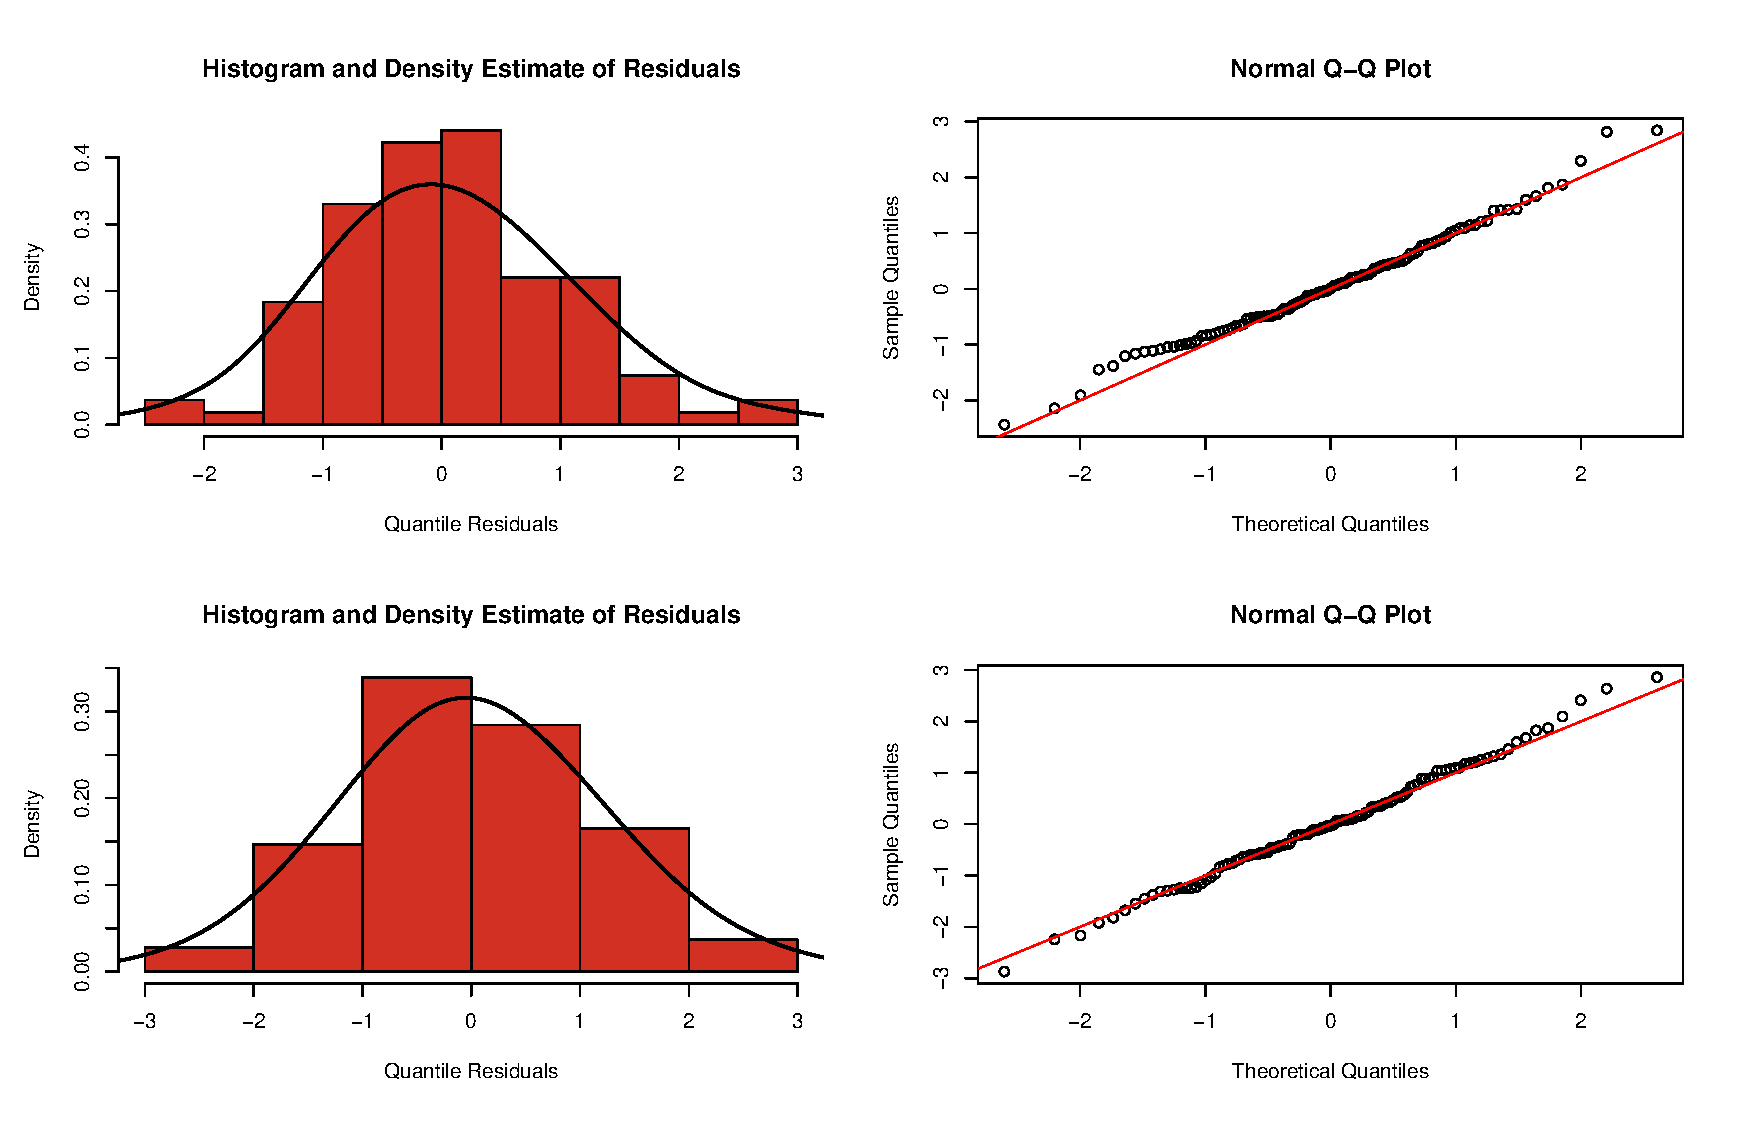
\includegraphics[width=0.9\linewidth]{figures/margin_estimates_kcc_68.eps}
  \caption{Estimation diagnostics for the response marginals KCC 6 \& KCC 8; \ac{GJRM} approach}
  \label{fig:margin_estimates_kcc_68}
\end{figure}
 



\begin{figure}[H]
\centering
  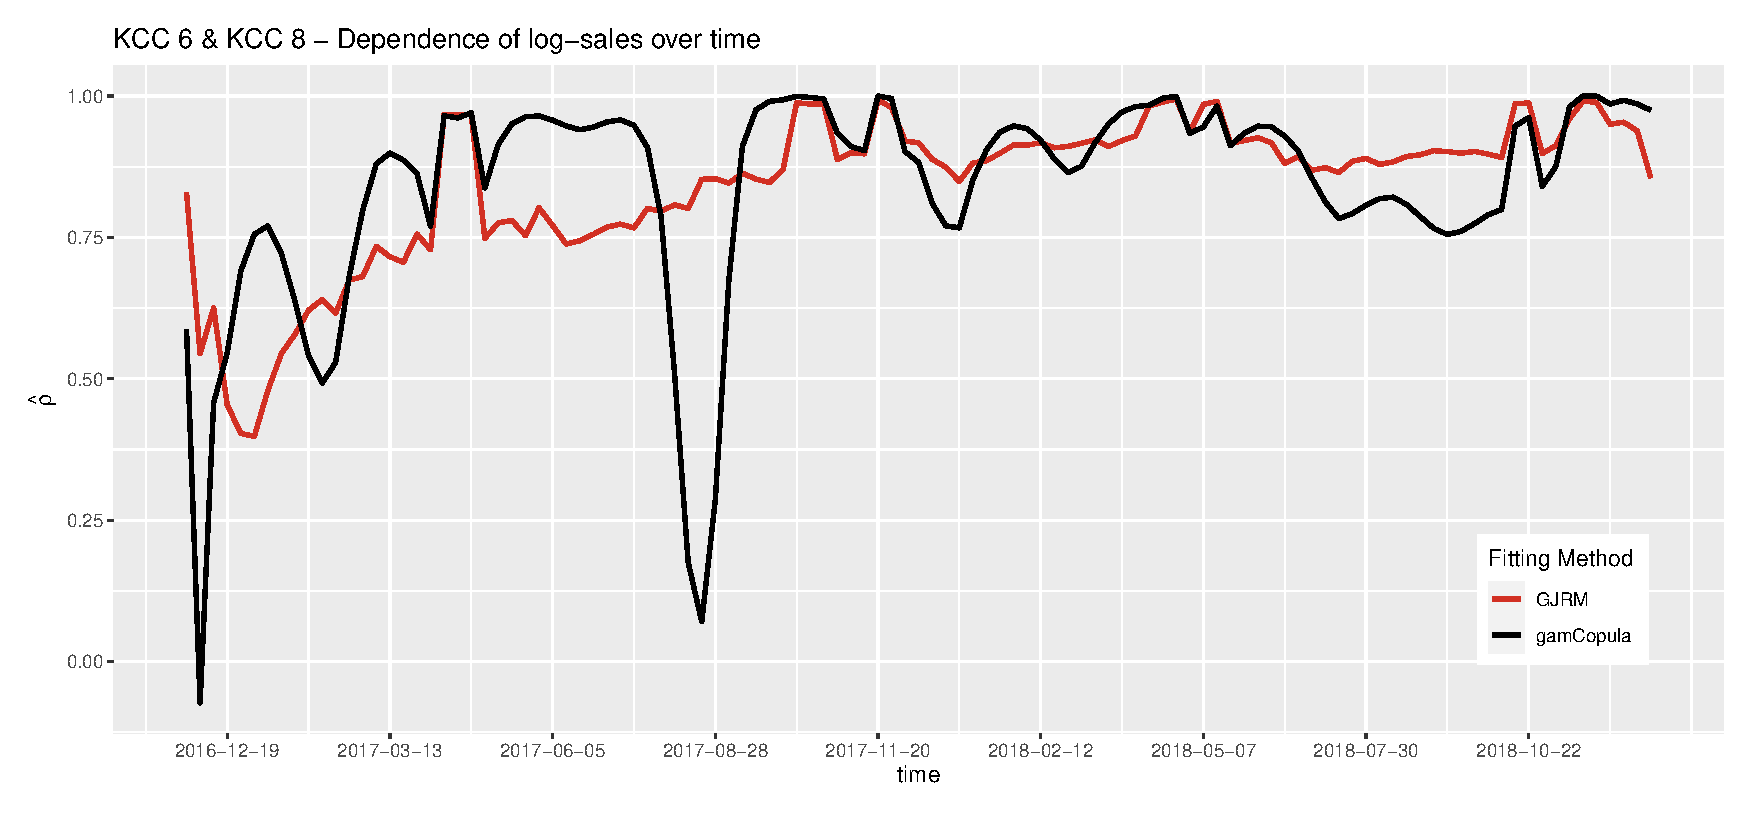
\includegraphics[width=0.9\linewidth]{figures/copula_parameters_68.eps}
  \caption{Estimated time-varying Pearson's correlation coefficients for the pair KCC 6 \& KCC 8}
  \label{fig:copula_parameters_68}
\end{figure}



In both correlations in \autoref{fig:copula_parameters_68} show an overall increasing trend from the start, which stabilizes somewhere in September of 2017. Both curves return positive values throughout the entire time span (except for the very start of the black one). Also, wider and heavier fluctuations occur in the gamCopula approach as opposed to the \ac{GJRM} method, which looks much smoother.